\documentclass[conference]{IEEEtran}
\IEEEoverridecommandlockouts

\usepackage{cite}
\usepackage{amsmath,amssymb}
\usepackage{graphicx}
\usepackage{booktabs}
\usepackage{url}
\usepackage[hidelinks]{hyperref}

\graphicspath{{figures/}}
\newcommand{\R}{R^2}

\begin{document}

\title{Music Emotion Recognition with Pretrained Audio Embeddings on DEAM\\[0.3em]
\large Progress Report}

\author{\IEEEauthorblockN{Can Y\"uzbey, Cem \"Ozkul, Efe Kumru, Emir Ceylan}
\IEEEauthorblockA{CS 415 Introduction to Deep Learning, Group 21, Sabanc\i\ University, Istanbul, Turkey\\
\{can.yuzbey, cem.ozkul, efe.kumru, emir.ceylan\}@sabanciuniv.edu}}

\maketitle

\begin{abstract}
We predict static valence and arousal for the 1{,}744 clips of DEAM. Following
the instructor's feedback, this report covers the data audit, an artist-grouped
10-fold protocol and the openSMILE baseline. The audit revealed two
undocumented defects in the 2013 part of DEAM: swapped static valence/arousal
labels and openSMILE features computed on the full song instead of the rated
excerpt. After correcting both, an SVR reaches $\R=0.38$ (valence) and $0.69$
(arousal) on artist-disjoint folds. We also show that per-clip listener
disagreement is almost unmeasurable with 10 raters, which clarifies what a
variance head can represent. MERT and the heteroscedastic head are in progress.
\end{abstract}

%======================================================================
\section{Problem and Motivation}
%======================================================================
We predict two continuous emotion scores per music clip, \emph{valence}
(negative to positive) and \emph{arousal} (calm to energetic), the axes of
Russell's circumplex model~\cite{russell1980}. Such scores support
emotion-aware music discovery. The task is hard for two reasons: labelled data
are scarce (DEAM has 1{,}744 rated 45\,s clips~\cite{aljanaki2017}), and
listeners disagree. Our aims, in the order requested in the feedback, are
(i) to show that a frozen pretrained encoder (MERT~\cite{li2024mert}, later
PANNs~\cite{kong2020}) beats hand-crafted openSMILE features~\cite{eyben2010}
with the same regression head, and (ii) to establish precisely what the
variance of a heteroscedastic head trained with Gaussian negative
log-likelihood (NLL) represents.

%======================================================================
\section{Related Work}
%======================================================================
Yang \emph{et al.}~\cite{yang2008} framed MER as regression on valence and
arousal with support vector regression (SVR) on hand-crafted descriptors,
still the usual baseline. DEAM comes from the MediaEval ``Emotion in Music''
tasks (2013--2015) and provides static and dynamic ratings plus openSMILE
features~\cite{aljanaki2017}; on it, Cheuk \emph{et al.}~\cite{cheuk2020}
report $\R\approx0.32$ (valence) and $0.64$ (arousal) for openSMILE-based
regressors. Pretrained encoders let us fit only a small head on DEAM:
PANNs~\cite{kong2020} are trained for general audio tagging, while
MERT~\cite{li2024mert} is self-supervised on music and reports strong emotion
results with frozen features. Their evaluations mostly use random splits, so
part of the gain may come from recognising artists.

Nix and Weigend~\cite{nix1994} introduced networks that predict a mean and a
variance trained with the Gaussian NLL; Kendall and Gal~\cite{kendall2017}
separate the noise such a head captures (aleatoric) from model uncertainty
(epistemic). Seitzer \emph{et al.}~\cite{seitzer2022} show that plain NLL lets
the variance down-weight hard samples and propose $\beta$-NLL. For MER,
Watcharasupat \emph{et al.}~\cite{watcharasupat2025} find that models learn
the mean rating but not how much listeners disagree; we examine why. Finally,
Bouthillier \emph{et al.}~\cite{bouthillier2021} show that split and seed
variance often exceed differences between models, which motivates our
cross-validated, paired comparisons.

%======================================================================
\section{Design Decisions}
%======================================================================
\textbf{Meaning of $\sigma$.} As the feedback noted, a variance fitted to the
\emph{mean} rating $\bar y_i$ of $n_i$ listeners is not the variance between
listeners. With $\mu_i$ the population mean and $f(x_i)$ the prediction,
\begin{equation}
\mathbb{E}[(\bar y_i - f(x_i))^2] = (\mu_i - f(x_i))^2 + s_i^2/n_i ,
\label{eq:sigma}
\end{equation}
i.e.\ model error plus averaging noise; listener spread $s_i$ enters only
divided by $n_i\approx10$. We therefore evaluate $\sigma$ as a predictive
uncertainty (calibration, rank correlation with $|e|$) and treat its relation
to $s$ as descriptive only. Since per-rater ratings exist, a head trained on
individual ratings is planned as a direct model of listener spread.

\textbf{Protocol.} Instead of one 70/15/15 split we use artist-grouped,
quadrant-stratified 10-fold cross-validation (seed 415); for test fold $k$,
fold $k{+}1$ is validation. Every clip is tested once, models are compared by
paired per-fold tests, and no artist appears in two folds. As the feedback
warned that fixed thresholds are optimistic, H1 is now decided relatively:
MERT must beat openSMILE \emph{with the same head} (ridge, then an MLP). We
report $\R$, RMSE and the concordance correlation coefficient (CCC) per
dimension, and PICP, NLL and $\rho(\sigma,|e|)$ for $\sigma$ models.

\textbf{Representations.} openSMILE: mean and standard deviation of DEAM's 260
frame-level descriptors over the excerpt (520-d). MERT-v1-95M: nine 5\,s
windows at 24\,kHz, all 13 layers cached, layer chosen on validation.

\textbf{Variance stability.} The heteroscedastic MLP bounds $\sigma$ softly,
$\sigma=\sigma_{\min}+(\sigma_{\max}-\sigma_{\min})\,\mathrm{sigmoid}(z)$ with
$\sigma_{\min}=0.01$ and $\sigma_{\max}=2\,\mathrm{sd}(y_{\text{train}})$,
avoiding hard clamps that kill gradients. The mean is warmed up with MSE before
switching to $\beta$-NLL ($\beta=0.5$; $\beta=0$ as comparison); early stopping
and model selection use plain validation NLL~\cite{seitzer2022}; and the share
of $\sigma$ near either bound is logged, with $>5\,\%$ flagged as unstable.
The reference is a constant $\sigma$ equal to the validation RMSE.

%======================================================================
\section{Experiments and Results}
%======================================================================
\textbf{Audit and split.} All 1{,}744 clips have valid labels, audio and
features; 10--20 raters per clip (median 10, 187 raters); 898 artists (1--23
songs each). The fold file passes an integrity test (each clip once, no artist
in two folds); folds hold 134--215 clips.

\textbf{Defect 1: swapped 2013 labels.} A first baseline gave $\R_A=0.29$ on
2013 but $0.69$ on 2014. Comparing static labels with the time-averaged dynamic
annotations of the same clips (Fig.~\ref{fig:swap}) shows that in 2013 static
valence matches dynamic \emph{arousal} ($r=0.96$) and vice versa ($0.95$),
while in 2014 the matching dimensions agree ($0.91$/$0.94$). Loudness confirms
this. We swap the 744 clips back.

\textbf{Defect 2: full-song features.} For 2013 the supplied openSMILE files
cover the whole song (up to 585\,s) while audio and ratings cover a 45\,s
excerpt. We crop them using the segment start in the metadata, verified on 21
clips against the audio energy (all within 0.5\,s). Table~\ref{tab:batch}
shows that the batch gap closes after both fixes.

\begin{figure}[t]
\centering
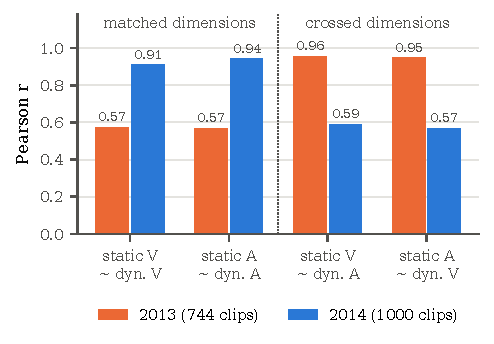
\includegraphics[width=0.92\columnwidth]{fig_va_swap}
\caption{Correlation of static labels with time-averaged dynamic annotations.
In 2013 the crossed dimensions agree: valence and arousal are swapped.}
\label{fig:swap}
\end{figure}

\begin{table}[t]
\centering
\caption{SVR $\R$ by batch before/after the label fix.}
\label{tab:batch}
\footnotesize
\begin{tabular}{@{}lcccc@{}}
\toprule
 & \multicolumn{2}{c}{supplied labels} & \multicolumn{2}{c}{corrected} \\
\cmidrule(lr){2-3}\cmidrule(l){4-5}
Batch ($n$) & $\R_V$ & $\R_A$ & $\R_V$ & $\R_A$ \\
\midrule
2013 (744)  & 0.61 & 0.29 & 0.37 & 0.65 \\
2014 (1000) & 0.38 & 0.69 & 0.43 & 0.74 \\
\bottomrule
\end{tabular}
\end{table}

\begin{table}[t]
\centering
\caption{openSMILE baselines on artist-grouped folds (mean $\pm$ SD over 10 folds).}
\label{tab:baseline}
\footnotesize
\setlength{\tabcolsep}{4pt}
\begin{tabular}{@{}llccc@{}}
\toprule
Head & Dim & $\R\uparrow$ & RMSE$\downarrow$ & CCC$\uparrow$ \\
\midrule
Ridge & V & 0.372$\pm$0.079 & 0.216$\pm$0.017 & 0.563$\pm$0.070 \\
      & A & 0.671$\pm$0.061 & 0.189$\pm$0.017 & 0.806$\pm$0.041 \\
SVR   & V & \textbf{0.379}$\pm$0.075 & \textbf{0.215}$\pm$0.012 & \textbf{0.565}$\pm$0.063 \\
      & A & \textbf{0.693}$\pm$0.045 & \textbf{0.183}$\pm$0.013 & \textbf{0.822}$\pm$0.029 \\
\bottomrule
\end{tabular}
\end{table}

\begin{figure}[t]
\centering
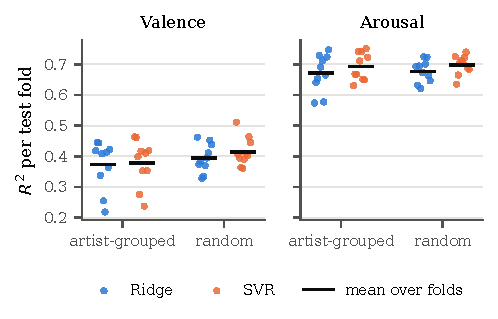
\includegraphics[width=0.92\columnwidth]{fig_baseline_folds}
\caption{Per-fold test $\R$ of the baselines on artist-grouped and random folds.}
\label{fig:folds}
\end{figure}

\textbf{openSMILE baseline.} Hyperparameters were chosen per fold on
validation RMSE (Table~\ref{tab:baseline}, Fig.~\ref{fig:folds}). The SVR
reaches $\R=0.38/0.69$, consistent with the $0.32/0.64$ of~\cite{cheuk2020}.
It beats ridge on arousal (8/10 folds, Wilcoxon $p=0.049$) but not on valence.
Random folds raise $\R_V$ by 0.035 but $\R_A$ by only 0.005, so artist
leakage mainly inflates valence. The noise ceiling of the mean rating is
$0.79/0.85$, leaving clear room for better representations.

\textbf{Listener disagreement.} Split-half reliability (500 random 5/5 rater
splits, corrected to 10 raters) is high for the mean rating ($0.79$/$0.85$)
but near zero for the listener standard deviation $s$ ($0.00$/$0.05$; $0.21$/$0.14$
after removing rater bias and scale). Moreover, model error is
\emph{negatively} related to $s$ (Spearman $-0.15$/$-0.10$, $p<10^{-4}$;
Fig.~\ref{fig:dis}): clips near the scale centre have more disagreement but
are easier to predict. A $\sigma$ that tracks the model's error, as
Eq.~\ref{eq:sigma} implies, therefore cannot be expected to track
disagreement, which explains the finding of~\cite{watcharasupat2025}.

\begin{figure}[t]
\centering
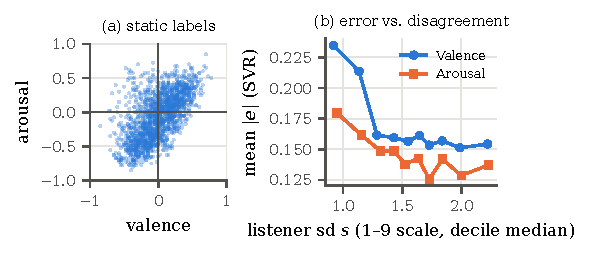
\includegraphics[width=0.92\columnwidth]{fig_labels_disagreement}
\caption{(a) Corrected labels. (b) SVR error per decile of listener spread $s$.}
\label{fig:dis}
\end{figure}

\textbf{Uncertainty reference and work in progress.} The constant-$\sigma$
reference is already calibrated on average (PICP$_{68}\approx0.68$,
PICP$_{95}\approx0.95$), so the heteroscedastic head must improve NLL and
error ranking to be useful. A prototype head runs end-to-end but was trained
on the uncorrected labels, so its results are not reported. The MERT
extraction script is ready; the cache was not complete at the time of writing.

%======================================================================
\section{Summary and Next Steps}
%======================================================================
We audited the data, built and verified an artist-grouped 10-fold protocol,
corrected two defects in DEAM 2013, established the openSMILE baseline
($\R=0.38/0.69$, CCC $=0.57/0.82$), quantified the artist effect, and showed
that listener disagreement is barely measurable, which fixes how $\sigma$ will
be interpreted. Next we will (1) train ridge and an MLP on MERT and compare
them fold by fold with openSMILE (H1); (2) rerun the heteroscedastic head on
corrected labels and report calibration, $\rho(\sigma,|e|)$, NLL against the
constant-$\sigma$ reference and stability logs, adding a seed ensemble; and
(3) then add PANNs and a head trained on individual ratings.

\bibliographystyle{IEEEtran}
\bibliography{refs}

\end{document}
